\documentclass[11pt]{article}
\usepackage[utf8]{inputenc}
\usepackage[T1]{fontenc}
\usepackage{graphicx}
\usepackage[export]{adjustbox}
\graphicspath{ {./images/} }
\usepackage{amsmath}
\usepackage{amsfonts}
\usepackage{amssymb}
\usepackage[version=4]{mhchem}
\usepackage{stmaryrd}

\begin{document}
The EUSIPA Classification

Structured products include a wide spectrum of offerings throughout the world that are difficult to categorize precisely. However, the EUSIPA has developed a valuable categorization that is partly summarized in this section. The EUSIPA (European Structured Investment Products Association) was founded in 2009 as a nonprofit association "to promote the interests of the structured retail investment products market." The EUSIPA publishes the EUSIPA Derivative Map, which categorizes structured products with two major classifications: investment products and leverage products. The Investment Products in the EUSIPA Derivative Map includes three major sub-categories: capital protection products, yield enhancement products, and participation products. The next four sections of this lesson briefly overview the three investment products' sub-categories and the leverage products category.

\section*{Capital Protection Structured Products}
The EUSIPA Derivative Map (May 2016) has five capital protection structured products, four of which are illustrated in the exhibit, Four Capital Protection Structured Products. In each diagram, the payoff of the structured product (the thicker, kinked line) is overlaid on the payoff of the product's underlying asset (the thinner, straight line). The underlying asset is often an equity index. Capital protection structured products tend to offer long call-option-like payoffs: downside protection, upside potential, and below-market interest income.

Uncapped Capital Protection

\begin{center}
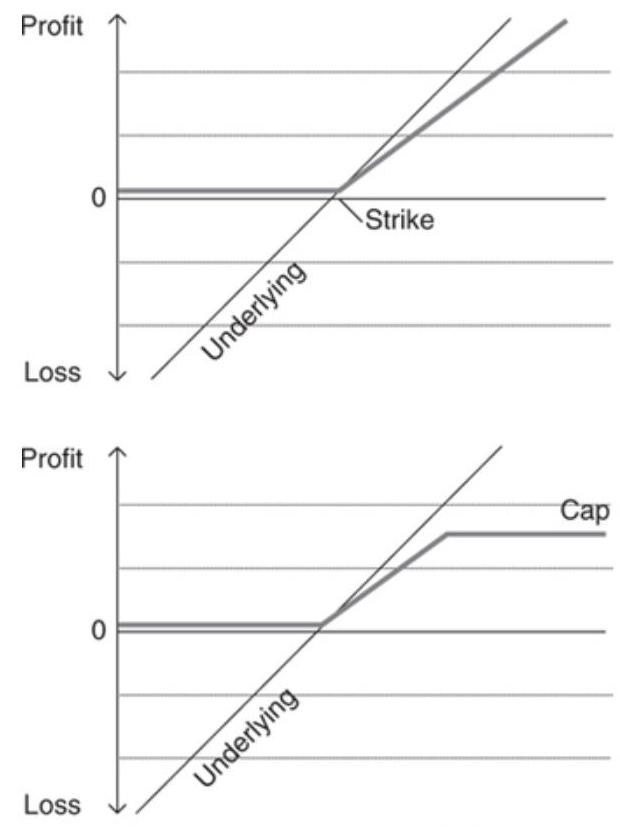
\includegraphics[max width=\textwidth]{2024_04_10_b75ef470ae043c0f718dg-2(1)}
\end{center}

Capped Capital Protection\\
Exchangeable Certificates\\
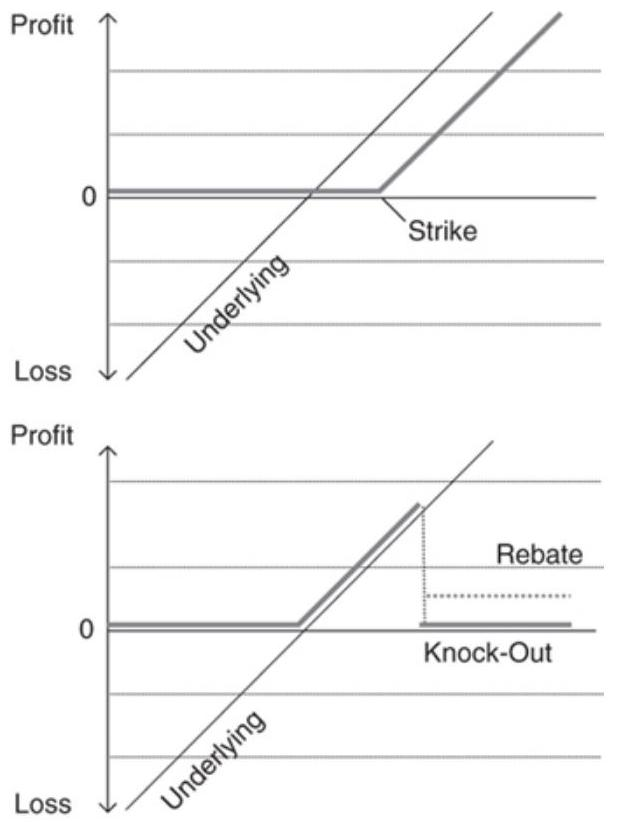
\includegraphics[max width=\textwidth, center]{2024_04_10_b75ef470ae043c0f718dg-2}

Capital Protection with Knock-Out

Four Capital Protection Structured Products

Source: EUSIPA Derivative Map (May 2016).

Note that the uncapped capital protection product offers great downside protection but has a less attractive upside potential than the equity index. Specifically, investors in this product gain only a portion of any profits generated by the underlying asset (i.e., they have a participation rate of less than $100 \%$ ). The exchangeable certificates offer downside protection and a $100 \%$ participation rate for profits, but the participation in profits does not take effect until there has been a prespecified increase in the value of the underlying index. The capped capital protection and capital protection structured products with a knock-out shown on the bottom of the Four Capital Protection Structured Products exhibit also offer only a portion of any upside profits generated by the underlying asset.

The full downside protection (principal protection) and the partial upside participation are the two key attributes to the four capital structured products in Four Capital Protection Structured Products exhibit and form an important concept discussed in greater detail at the end of the session: Issuers of these types of structured products cannot earn competitive rates of return by offering products that guarantee investors uniformly superior payoffs, such as full upside participation with no downside risk. Some structured products, such as collateralized loan obligations in which the issuing institution (e.g., a bank) is gaining advantages such as freeing up regulatory capital, may be willing to offer attractive returns to investors who purchase the loans. The equity-linked structured products discussed in this session are issued to provide compensation to the issuer for creating products that investors perceive as enhancing their expected utility.

In essence, capital protection structured products are similar to long call options. The buyer usually compensates the issuer for this call option by accepting little or no interest income on the buyer's investment. To varying extents, investing in these products is similar to purchasing call options through the sacrifice of current income.

\section*{Two Yield Enhancement Structured Products}
The EUSIPA Derivative Map (May 2016) has seven yield enhancement structured products, two of which are illustrated in Two Yield Enhancement Structured Products. Yield enhancement structured products tend to offer short put-option-like payoffs with full downside exposure, capped upside potential, and abovemarket interest income (i.e., yield enhancement).

Note that the discount certificate payoff diagram is identical to a short put option. However, the barrier discount certificate has a range that contains two potential payoffs: one in the case that a barrier is reached (the horizontal solid line) and one in the case that the barrier is not reached (the dotted line). Barrier options are a common component of complex structured products.

Discount Certificates

\begin{center}
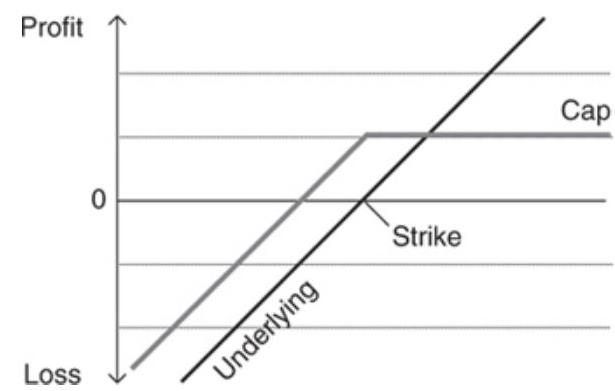
\includegraphics[max width=\textwidth]{2024_04_10_b75ef470ae043c0f718dg-3(1)}
\end{center}

Barrier Discount Certificates

\begin{center}
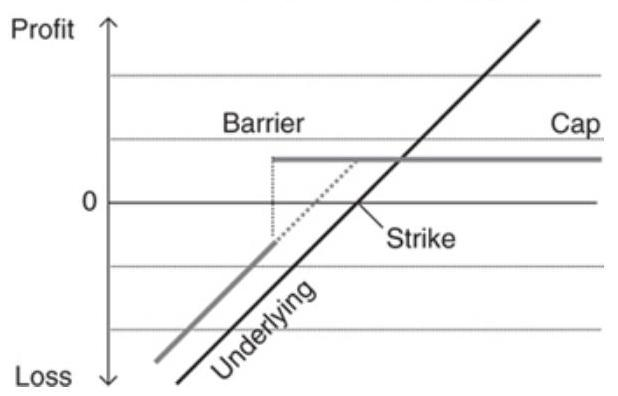
\includegraphics[max width=\textwidth]{2024_04_10_b75ef470ae043c0f718dg-3(2)}
\end{center}

Two Yield Enhancement Structured Products

Source: EUSIPA Derivative Map (May 2016).

\section*{Two Participation Structured Products}
The EUSIPA Derivative Map (May 2016) has five participation structured products, two of which are illustrated in the exhibit, Participation Structured Products. Participation structured products tend to offer exposures (bull or bear) to the underlying index (or assets) that are not capped in terms of potential profits or losses (i.e., in either the bull or bear scenarios). Therefore, participation structured products differ from capital protection products (that tend to be long call options) or yield enhancement products (that tend to be short put options).

Tracker Certificates

\begin{center}
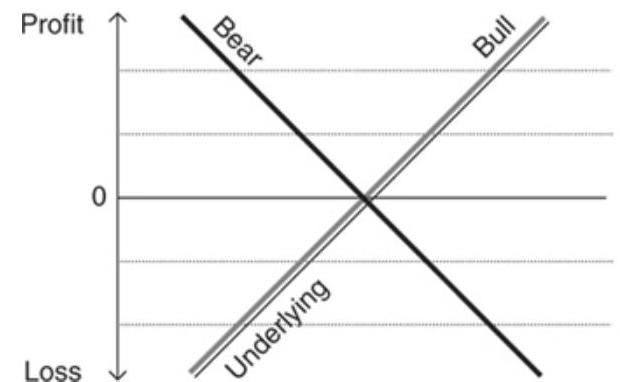
\includegraphics[max width=\textwidth]{2024_04_10_b75ef470ae043c0f718dg-3(3)}
\end{center}

\begin{center}
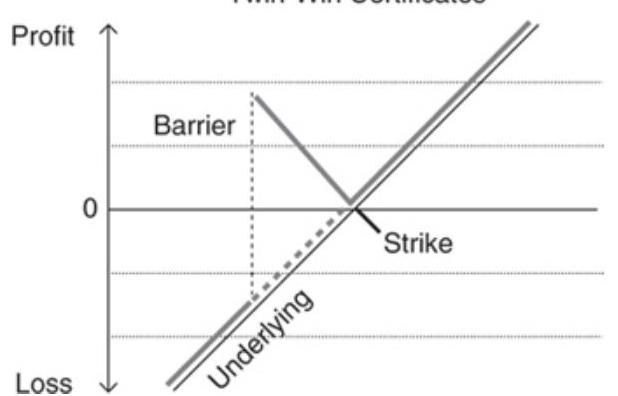
\includegraphics[max width=\textwidth]{2024_04_10_b75ef470ae043c0f718dg-3}
\end{center}

\section*{Participation Structured Products}
Source: EUSIPA Derivative Map (May 2016).

The tracker certificates depicted on the left side of Participation Structured Products exhibit offer full exposures-bull or bear-to the underlier. The purpose for a buyer to use this tracker product rather than simply establish a long or short position directly in the cash market for the index may be to obtain the exposures inside one of the various wrappers discussed earlier in this session.

The twin-win certificates on the right side of Participation Structured Products offer absolute return exposures over a limited range similar to a long position in an option straddle. As with many other long-option-like structured products, the cost of the long option will be embedded in the product through reduced income.

\section*{Four Leverage Structured Products}
The EUSIPA Derivative Map (May 2016) has seven leverage structured products, four of which are illustrated in Leverage Structured Products. Leverage structured products have three subcategories: leverage without knock-outs, leverage with knock-outs, and constant leverage. They tend to offer exotic exposures that do not fit neatly in the map's investment structured product categories.

The top two products in Leverage Structured Products use knock-outs to create limits to profits and losses, thereby providing targeted exposures over limited ranges of the underlier. The leverage product in the lower left corner depicts offerings of bull spreads and bear spreads, whereas the bottom right corner product depicts pure leveraged products that offer participation rates (bull or bear) in excess of $100 \%$.

This brief survey of types of structured products demonstrates the tremendous variety of exposures available. It should be noted that actual products are often far more complex than the exposures discussed in this section. The structured products focused on the retail market are designed by issuers to meet the preferences, predictions-and, some would argue, behavioral biases-of non-institutional investors. With the tremendous spectrum of risk exposures available, and perhaps with the high degree of complexity, at least some of the products would appear to be attractive to any investor with a "market view." Unfortunately, that market view may emanate more from an emotional reaction to the casual observation of recent market performance than from sound economic reasoning and sound analysis of longterm historical data.

\begin{center}
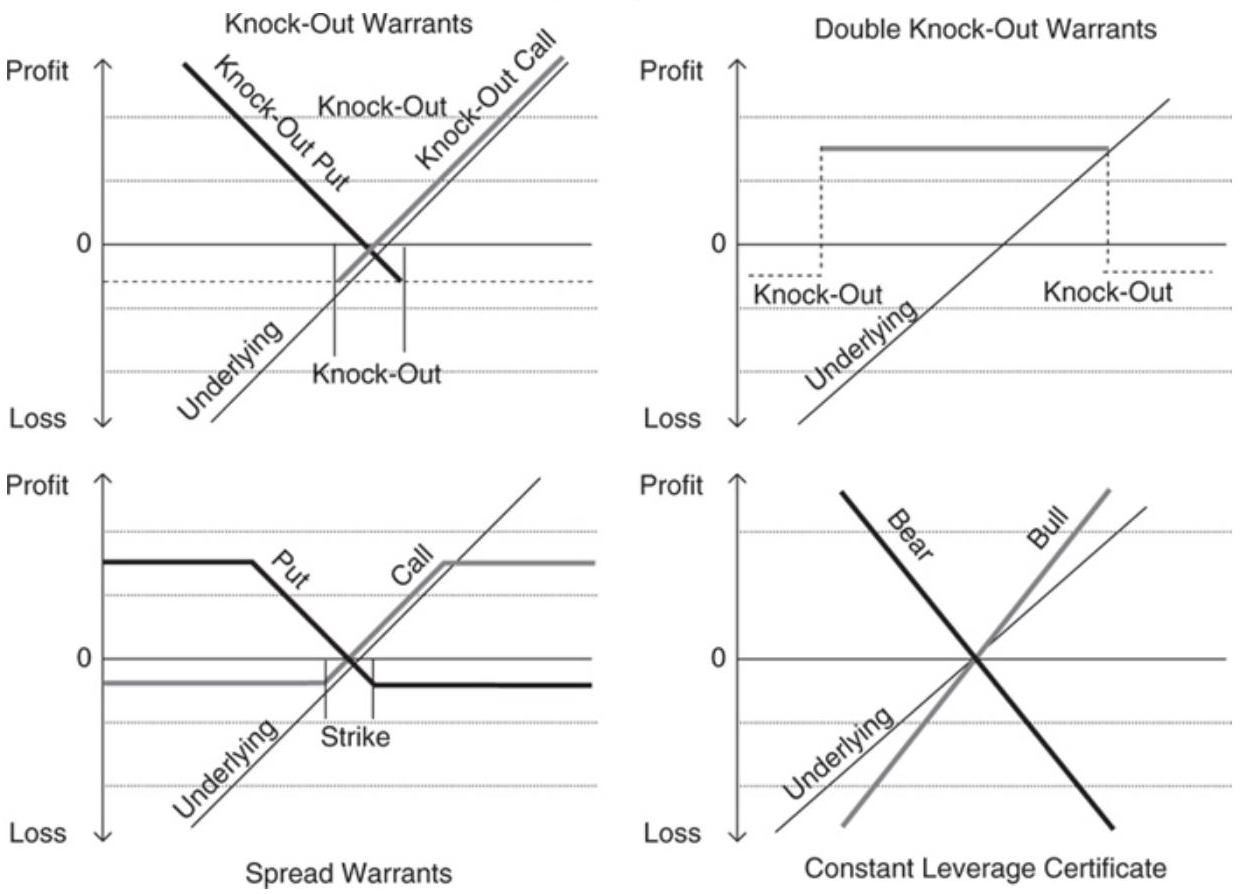
\includegraphics[max width=\textwidth]{2024_04_10_b75ef470ae043c0f718dg-4}
\end{center}

Leverage Structured Products


\end{document}